% Joint report, DSA4212 group project. DRAFT assembled from the two parts:
%   Part A (multimodality): written from multimodality/docs/report_log.md; numbers checked against
%   multimodality/results/summary/.
%   Part B (geometry): condensed from geometry/report/report.tex; numbers from geometry/results/.
% Every section must be rewritten by its author in their own words before submission (see %% AUTHOR notes).
\documentclass[10pt,a4paper]{article}
\usepackage[margin=1.8cm]{geometry}
\usepackage[T1]{fontenc}
\usepackage[utf8]{inputenc}
\usepackage{lmodern}
\usepackage{amsmath,amssymb}
\usepackage{graphicx}
\usepackage{booktabs}
\usepackage[numbers,sort&compress]{natbib}
\usepackage{xcolor}
\usepackage[colorlinks=true,linkcolor=black,citecolor=black,urlcolor=blue]{hyperref}
\setlength{\parskip}{3pt}
\setlength{\parindent}{0pt}
% Compact lists and small captions without extra packages (TinyTeX/Overleaf-safe).
\let\olditemize\itemize
\renewcommand{\itemize}{\olditemize\setlength{\itemsep}{1pt}\setlength{\parskip}{0pt}\setlength{\topsep}{2pt}}
\makeatletter\renewcommand{\@makecaption}[2]{\vskip 4pt{\small\textbf{#1.} #2\par}}\makeatother
\newcommand{\ci}[2]{[#1,\,#2]}
\newcommand{\dec}{\,decades}

\title{\vspace{-1.3cm}Does the model fit the landscape?\\
Shape and scale in Bayesian optimisation and CMA-ES\vspace{-0.3cm}}
\author{Isaac Soong Hong Wei (A0272752B), Paul Ng Yin Chen (A0272249Y)\\[2pt]
\small Repository: \url{https://github.com/isaacsoong055/DSA4212}}
\date{\vspace{-0.7cm}}

\begin{document}
\maketitle

\begin{abstract}
\noindent
Bayesian optimisation (BO) and CMA-ES both carry an implicit model of the landscape: CMA-ES a Gaussian
search distribution with a covariance (its shape) and a step size (its scale), BO a Gaussian-process
surrogate whose kernel metric and lengthscales play the same two roles. We test one explanation in two
settings: a method succeeds when its model's shape and scale can match the problem, whatever its family.
\emph{Part A (multimodality)} asks
whether the model's scale lets a method \emph{find} and then \emph{refine} a narrow distant basin: neither
default method finds it; CMA-ES's step size cannot do both jobs at once, and BO succeeds once its lengthscale
is capped (1/50 to 44/50 on fresh seeds) while acquisition tuning helps far less. \emph{Part B (geometry)}
asks whether the model can \emph{tilt}: on rotated, ill-conditioned valleys diagonal CMA-ES, the ARD kernel
and TuRBO's axis-aligned trust region all fail, while their tilting counterparts do not, once BO's own fitting
failures are removed. In both parts the decisive
BO changes were to the model fit, not the acquisition function. All results are in 2-D and pre-registered
predictions are reported whether they held or failed.
\end{abstract}

%=====================================================================
\section{Introduction}
%=====================================================================
%% AUTHORS: joint section, rewrite together in your own words.
\subsection{Motivation and the two methods}
Many optimisation problems give only function values: tuning a model's hyperparameters, calibrating a
simulator, choosing a design. There are no gradients, and each evaluation can cost a training run or a
simulation, so a method must decide where to evaluate next from the values it has seen, and its budget is
counted in evaluations. Bayesian optimisation (BO) and the covariance matrix adaptation evolution strategy
(CMA-ES) are two of the most widely used methods for this setting, and they embody opposite design choices:
BO models the function, while CMA-ES adapts a search distribution.

\emph{BO} \citep{frazier2018tutorial} fits a Gaussian-process (GP) surrogate to all evaluations so far. Its
kernel encodes smoothness and lengthscales, and its posterior gives a prediction and an uncertainty everywhere.
An acquisition function, such as expected improvement (EI), turns these into the next point, trading off
exploiting good predictions against exploring uncertain regions. \emph{CMA-ES} \citep{hansen2016tutorial}
samples a population of $\lambda$ candidates from a Gaussian $\mathcal N(m,\sigma^2C)$, ranks them, moves the
mean towards the best, and adapts the covariance $C$ and the step size $\sigma$ from successful steps. It uses
only the ranking of the values. The basic trade-off follows: BO is sample-efficient because it uses every value
through a global model, but each step is expensive (fitting the GP grows cubically with the number of points)
and its success depends on that model being right; CMA-ES needs more evaluations but each step is nearly free,
and it learns the \emph{local} geometry of the problem.

\subsection{What the literature says, and what it leaves open}
Our questions came from the readings. Hansen's tutorial \citep{hansen2016tutorial} states the invariances
CMA-ES is designed to have: to any order-preserving transformation of $f$, and to rotations and other linear
maps of the search space provided the initial conditions are mapped too; its covariance comes to approximate
the inverse Hessian on a convex quadratic. This raised the question of which invariances survive in practice
and whether a model that cannot rotate pays for it. Restart schemes that grow or mix the population size
(IPOP, BIPOP \citep{auger2005ipop,hansen2009bipop}) were introduced for multimodal functions, which raised the
question of whether population and restarts help find a narrow basin. TuRBO \citep{eriksson2019turbo} restricts
BO's search to local trust regions whose sides are set per coordinate from the ARD lengthscales, an axis-aligned
shape;
COCO \citep{hansen2021coco} sets the benchmarking practice we follow (budgets in evaluations, random instances,
targets and intervals).

The literature also shows that BO's results depend on settings that are rarely reported. Hvarfner et al.
\citep{hvarfner2024vanilla} argue that BO's poor high-dimensional performance owes much to its lengthscale
prior, and that a dimension-scaled prior makes plain BO competitive. Ament et al. \citep{ament2023logei} show
that EI's values and gradients vanish numerically, so the acquisition optimiser can fail; and Siivola et al.
\citep{siivola2018boundary} show that GP-based BO over-explores the boundary of the search box. A comparison of
``BO against CMA-ES'' run with library defaults therefore mixes the family with hidden choices: kernel fitting,
lengthscale bounds, noise handling, step size. What remains open is which of those properties actually
decides success.

\subsection{Problem formulation}
\emph{Research question.} When BO and CMA-ES succeed or fail on a black-box problem, which property of the
method decides the outcome, and does it matter more than the choice of family?

\emph{Guiding hypothesis.} Each method carries an implicit model of the landscape. For CMA-ES it is the search
distribution: the covariance sets its \emph{shape} (orientation and relative stretch) and the step size its
\emph{scale}. For BO it is the GP: the kernel metric sets the shape (a full metric, or the diagonal ARD metric)
and the lengthscales the scale. A method succeeds when its model can match the landscape's shape (orientation,
conditioning) and scale (the size of the features it must find and resolve), and fails when a restriction or a
fitting failure prevents it, whichever family it belongs to.

\subsection{Shared experimental approach}
Both parts fix a budget counted in objective evaluations, with initial designs and restarts included; run
every variant on the same seeds, so comparisons are paired; change one setting at a time against a baseline;
and commit their predictions to the repository before the runs that test them, reporting each as held, partly
held or failed. A method's recommendation is its best evaluated point, judged on the true objective: in Part A
by whether its regret reaches a success threshold, in Part B by its regret in decades of $\log_{10} f$. With
noisy evaluations the recommended point is scored on the noise-free objective, and several recommendation
rules are compared. Uncertainty is given as 95\% intervals (Wilson and Newcombe intervals for success rates;
paired bootstrap intervals over instances for regret). The two parts use different budgets, measures and BO
implementations (BoTorch \citep{balandat2020botorch}; NumPy/SciPy), so their numbers are never put on common
axes.

\subsection{The two directions}
\emph{Part A, multimodality} (Isaac Soong), asks whether each method can \emph{find} a narrow, distant global
basin and then \emph{refine} it, within 300 evaluations. It varies CMA-ES's population size, restarts and step
size, and BO's acquisition function, GP fitting settings and kernel, on a decoy bowl with a narrow Gaussian well
(whose width and distance are varied), with a sphere as a unimodal control and Rastrigin and Schwefel as
validation functions.

\emph{Part B, geometry and parameterisation} (Paul Ng), asks whether a method's model can \emph{tilt} to a
rotated, ill-conditioned valley, and which theoretical invariances survive the implementation. It varies the
conditioning and rotation of the problem and whether each method's model can rotate (full against diagonal
covariance; full against ARD kernel metric; a rotated against an axis-aligned trust region), and also tests
changes of units, monotone transformations of $f$, the box boundary and noisy evaluations, on ellipsoids,
Rosenbrock (COCO f8/f9 \citep{hansen2009bbobfunctions}) and a noisy quadratic, within 200 evaluations.

\subsection{Preview of findings and contributions}
In Part A neither default method finds the well (CMA-ES 0/50 runs, BO 5/50). For CMA-ES, a larger population
and restarts change how often the well is touched but not success, because one step size cannot both find the
well and refine it. For BO, capping the GP lengthscale raises success to 39/50 (44/50 on fresh seeds), while
tuning the acquisition function reaches at most 17/50. In Part B, the axis-restricted version fails under
rotation in both families (diagonal CMA-ES solves no instance between $30^\circ$ and $60^\circ$; BO with ARD
loses 2.0 decades), but this became visible for BO only after a fitting failure that stalled every BO run was
diagnosed and fixed; the result then held across two kernels, two acquisition searches and a TuRBO-style trust
region. CMA-ES's rank invariance survives exactly; BO has neither invariance.

Together the parts contribute a tested account of shape and scale across both families; the shared, unplanned
finding that BO's decisive fixes were to the \emph{model fit}, not to the acquisition function; and a set of
negative and surprising results reported as such: pre-registered predictions that failed, an initial negative
result that turned out to be a fitting failure, a boundary trap, and BO runs that do not repeat bit for bit.

\emph{Roadmap.} Section~\ref{sec:partA} presents Part A and Section~\ref{sec:partB} Part B, each as question,
set-up, results and caveats. Section~\ref{sec:synth} draws the two together and states the limitations.

%=====================================================================
\section{Part A: finding and refining a narrow basin (multimodality)}\label{sec:partA}
%=====================================================================
%% AUTHOR: Isaac Soong. Written from multimodality/docs/report_log.md; rewrite in your own words.
\textbf{Question and predictions.} At a fixed budget of $N=300$ evaluations, how do population size, restarts,
step size and acquisition and surrogate choices change the probability of finding a narrow, distant global basin,
and why? Predictions H1--H6 and M1--M3 were committed before any optimiser result was inspected; BO1--BO13 and
CMA1--CMA6 were added later, each before the experiment that tested it, except BO1 (post hoc, labelled as such).

\textbf{Set-up.} The primary landscape is a broad decoy bowl with a narrow, deep Gaussian well,
$f(x)=\lVert x-c\rVert^2/s-A\exp(-\lVert x-x_g\rVert^2/2w^2)$ with $c=0$, $s=10$, $A=4$, width $w=0.3$, the
well at $(3,3)$ (Fig.~\ref{fig:land}), on $[-5,5]^2$. A run succeeds when its regret falls to $\varepsilon=0.05$,
a threshold chosen from random sampling alone. CMA-ES is the \texttt{cma} library (default $\lambda=6$,
$\sigma_0=2$, start $x_0\sim U[-4,4]^2$); BO is BoTorch GP-EI (Mat\'ern-5/2, 10 initial points, refit every 5
evaluations, lengthscale upper bound 20, fixed noise $10^{-6}$). Each variant changes one setting and uses seeds
1000--1049; success rates carry Wilson intervals and differences Newcombe intervals.

\begin{figure}[t]
\centering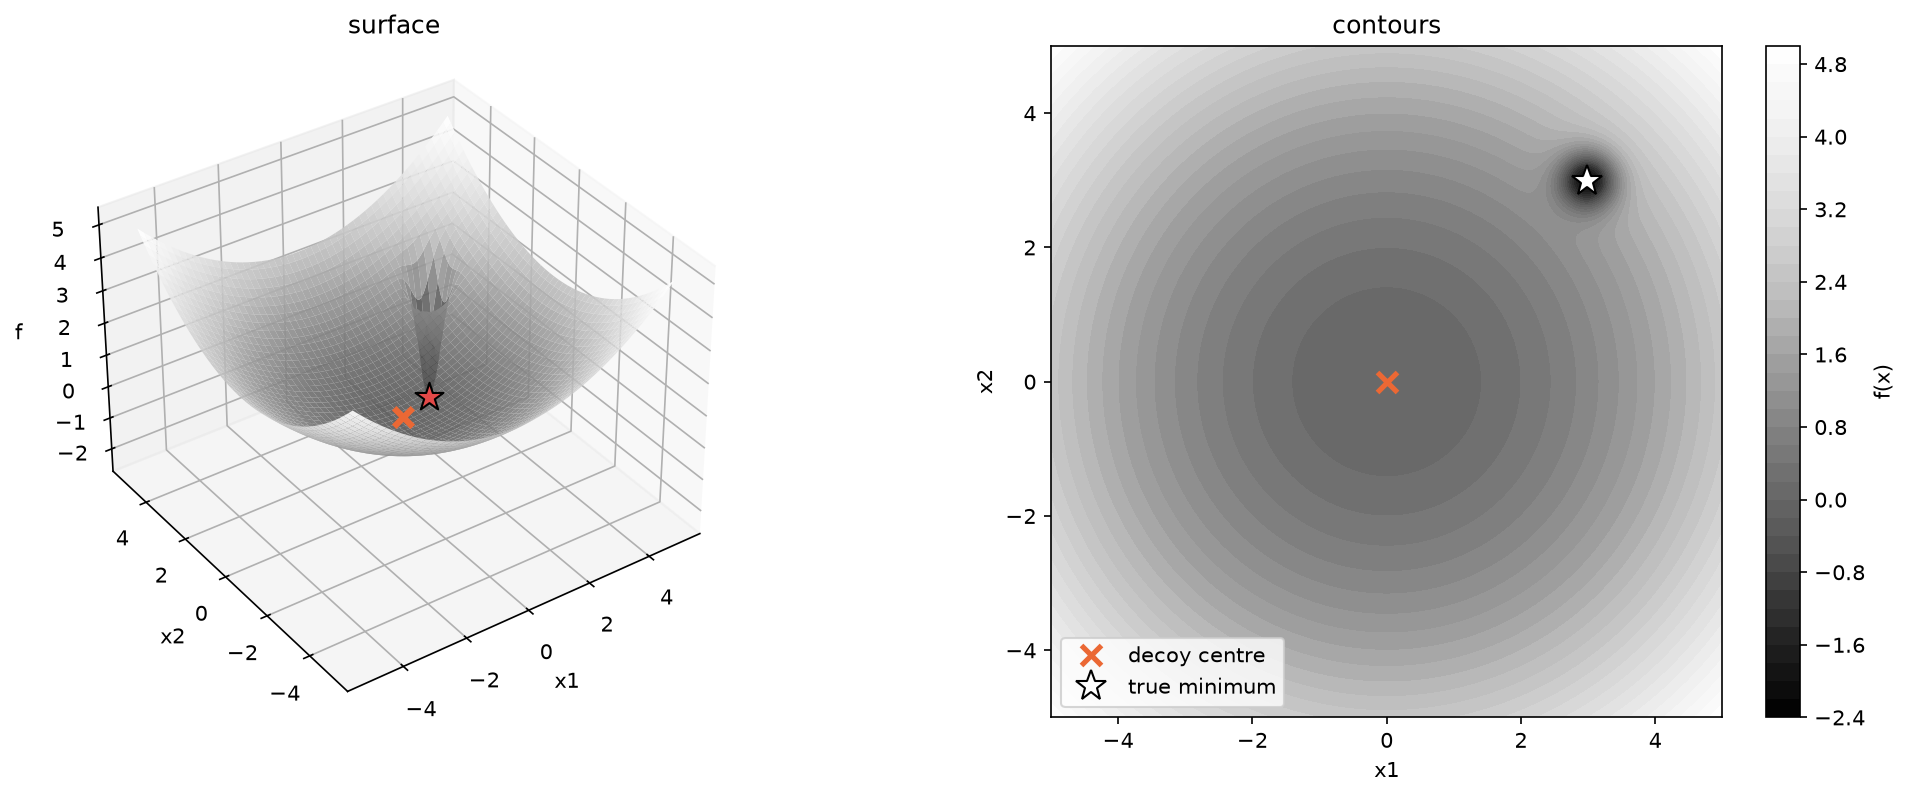
\includegraphics[width=0.7\linewidth]{figures/mm_landscape.png}
\caption{Part A. Primary landscape: a decoy bowl centred at the origin and a narrow global well at $(3,3)$, $w=0.3$.}
\label{fig:land}
\end{figure}

\textbf{Baselines (Exp 0).} Neither default finds the well: CMA-ES 0/50, BO 5/50, random sampling 2/50, with
pairwise-overlapping intervals. CMA-ES's $\sigma$ falls below 0.2 by generation 19 (median) and from evaluation 100
on at least 97.5\% of its samples lie within 0.5 of the decoy centre (H1 supported). BO's lengthscale runs to its
upper bound in 42 of 50 runs, none of which succeeds, and in the 45 failures no sample ever enters the well. Both
fail at \emph{discovery}, not refinement: every BO run that sampled the well succeeded.

\textbf{CMA-ES: population, restarts and step size (Exps 1--3).} A larger population raises the number of runs that
touch the well (1, 7 and 13 of 50 for $\lambda=6,12,24$) but success stays 0/50 at every $\lambda$, also with five
times the budget (H2 contradicted). IPOP and BIPOP \citep{auger2005ipop,hansen2009bipop} are identical at this
budget, because only one restart fits, and also give 0/50 (H3 contradicted on success). The step size explains why
(Fig.~\ref{fig:sig}): from a start 1.0 from the well, $\sigma_0=0.3$ succeeds in 33/50 runs and the default
$\sigma_0=2$ in 2/50 ($+0.62$ \ci{+0.45}{+0.74}), while from a random start no $\sigma_0$ exceeds 1/50. A mean trace
shows the mechanism: with $\sigma_0=2$, a single well sample is outvoted by the other selected points on the bowl,
which drag the mean back to the decoy. Finding the well needs a large $\sigma$ and refining it a small one, and
the default has to choose.

\begin{figure}[t]
\centering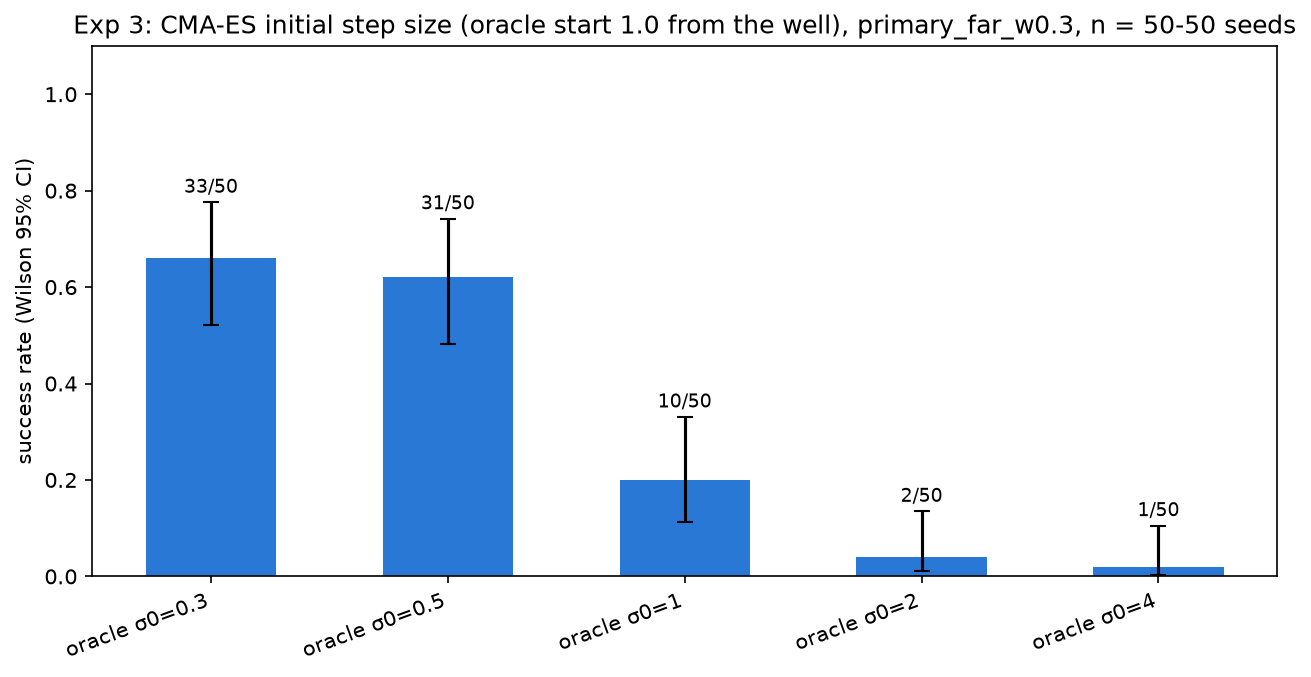
\includegraphics[width=0.66\linewidth]{figures/mm_exp3_oracle.png}
\caption{Part A, Exp 3. CMA-ES success against initial step size from a start 1.0 from the well (a diagnostic of
refinement, not a method comparison).}
\label{fig:sig}
\end{figure}

\textbf{BO: acquisition against model fit (Exps 4--7).} Exploration in EI helps a little: $\xi=0.1$ reaches 17/50
($+0.24$ \ci{+0.08}{+0.39} over $\xi=0$), and larger $\xi$ touches the well more often but refines it less (17/45 to
3/42 given a touch). LCB ($\beta$ from 0.5 to 32), Thompson sampling and BoTorch's default MAP recipe all stay at 3--4/50.
The model fit matters far more (Fig.~\ref{fig:fit}): capping the lengthscale at 1 gives 39/50 ($+0.68$
\ci{+0.51}{+0.79}), because the default fit runs to the bound and the search stays near the bowl centre, while a cap makes
it sweep the box (about 100 of 100 grid cells visited, against 10). The cap has an optimum: 0.25 drops back to 6/50.
Changing the kernel at the default cap changes nothing; at cap 1 RBF matches Mat\'ern-5/2 (39/50) but the rougher
Mat\'ern-3/2 and 1/2 collapse (6 and 3/50) by failing to discover the well.

\begin{figure}[t]
\centering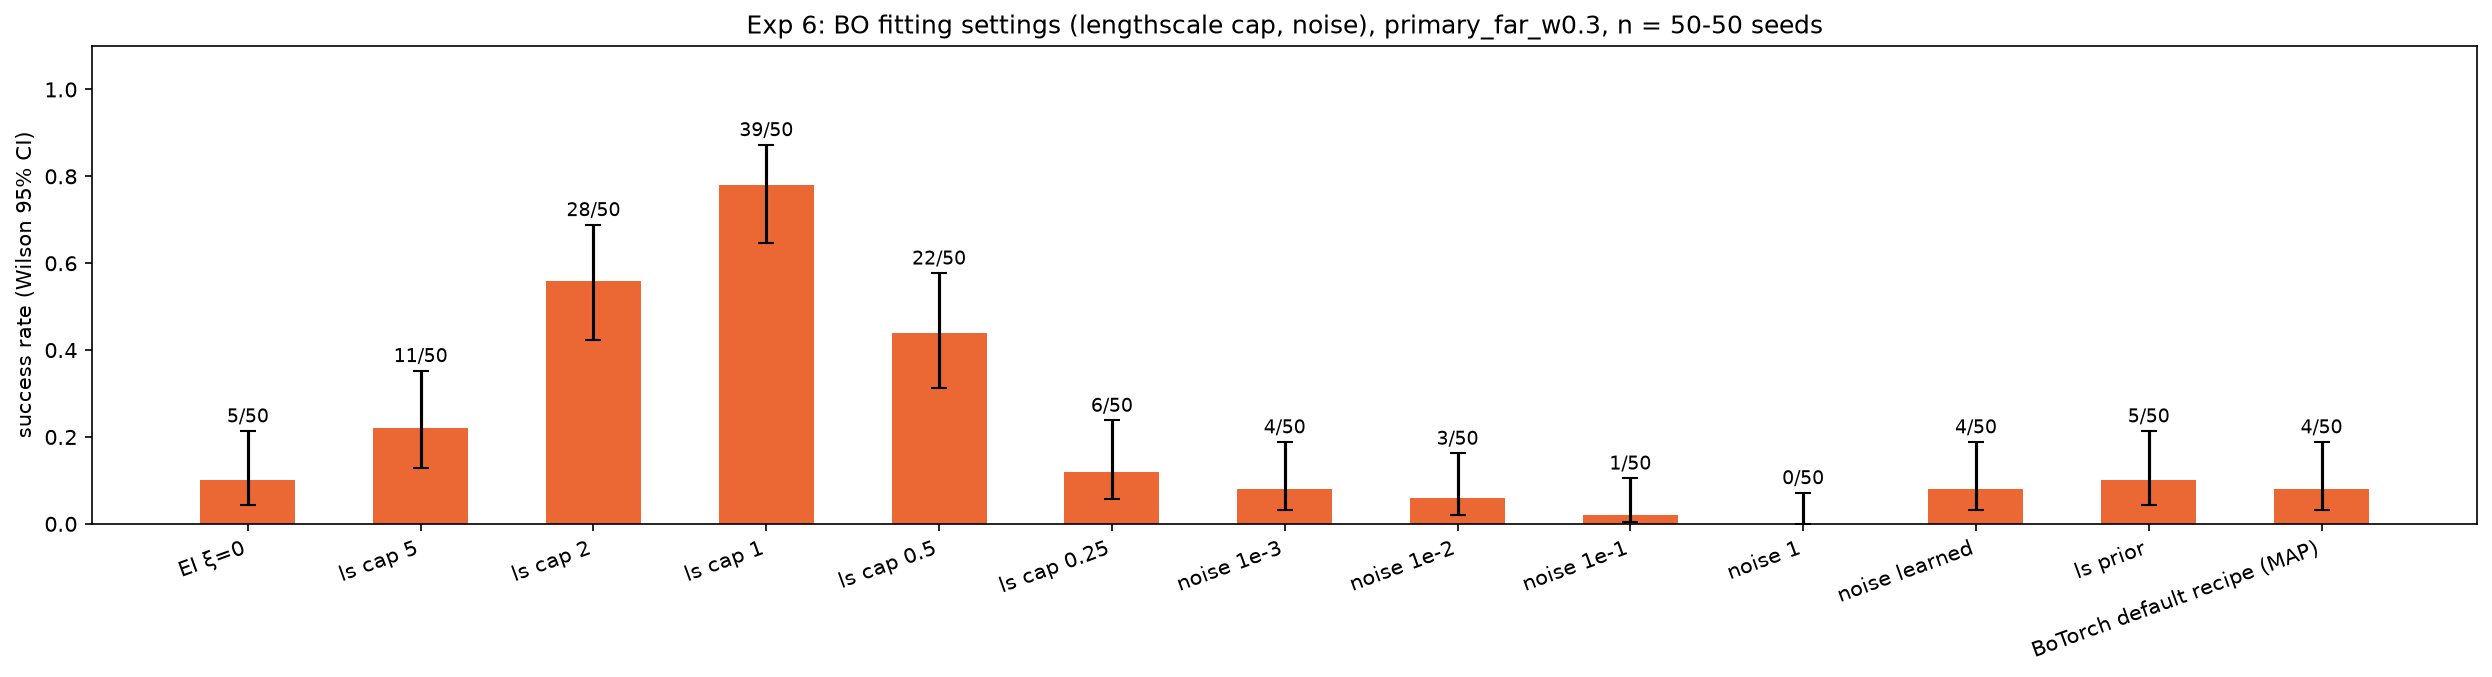
\includegraphics[width=\linewidth]{figures/mm_exp6_fitting.png}
\caption{Part A, Exp 6. BO fitting settings changed one at a time: lengthscale cap and noise level (BoTorch, $N=300$).}
\label{fig:fit}
\end{figure}

\textbf{Width, control and validation (Exps 8--10).} Across well widths (Fig.~\ref{fig:width}) the capped BO,
evaluated on fresh seeds 2000--2049 to avoid selection bias, succeeds in 44/50 at $w=0.3$ and 50/50 at $w=0.6$ and
1.0, against 1, 10 and 39/50 for default BO; CMA-ES needs a wide well (35/50 at $w=1.0$, 0/50 at $w=0.3$), and the
best CMA-ES variant ($\sigma_0=1$) gives no gain at any width. On a near well, default CMA-ES beats default BO (30 against
13/50 at $w=0.3$). The capped BO has a cost on a unimodal sphere (regret $8.9\times10^{-4}$ against $1.2\times10^{-6}$
at evaluation 100), and a larger $\lambda$ worsens CMA-ES there (H5 supported). On Rastrigin and Schwefel the cap's gain
is small and uncertain, and BO is far stronger than CMA-ES on Schwefel (16/20 default, 20/20 capped, against at most
8/50); whether $\lambda$ helps more on Rastrigin than on Schwefel (H6) could not be distinguished.

\begin{figure}[t]
\centering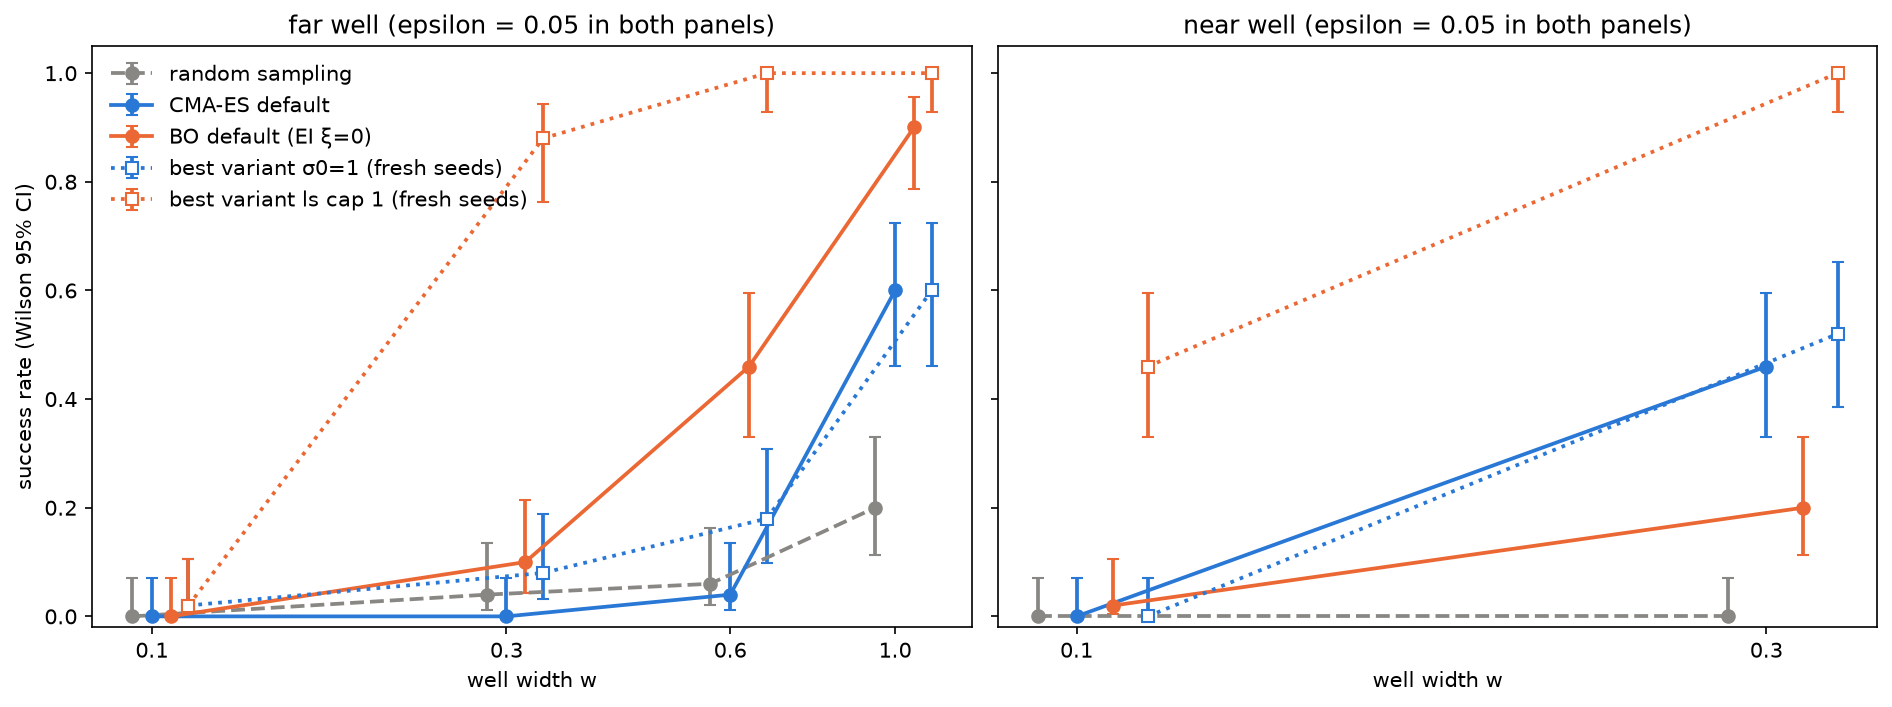
\includegraphics[width=0.9\linewidth]{figures/mm_exp8_width.png}
\caption{Part A, Exp 8. Success against well width for the defaults and the best variants (fresh seeds),
far and near well.}
\label{fig:width}
\end{figure}

%=====================================================================
\section{Part B: can the search tilt? (geometry and parameterisation)}\label{sec:partB}
%=====================================================================
%% AUTHOR: Paul Ng. Condensed from geometry/report/report.tex; rewrite in your own words.
\textbf{Question and predictions.} Near a minimum $f\approx f^*+\tfrac12h^\top Hh$. The Hessian's eigenvalues
are the curvatures; their ratio $\kappa$ is the conditioning (a narrow valley when large); its eigenvectors
are the valley's orientation, which a rotation changes without changing $\kappa$. A full covariance
(CMA-ES) or a full kernel metric $M=LL^\top$ (BO) can align with a rotated valley; a diagonal covariance,
the standard ARD kernel and TuRBO's axis-aligned trust region \citep{eriksson2019turbo} cannot. We predicted
that (i) each axis-restricted method pays a penalty under rotation that its tilting counterpart does not,
(ii) only when the problem is both ill-conditioned and rotated, and (iii) the tilting version pays a small
price when no tilt is needed.

\textbf{Set-up.} 2-D ellipsoids with log-spaced eigenvalues from 1 to $\kappa$, the optimum on a radius-2
sphere, aligned or Haar-rotated, 15 instances (COCO-style; seed = instance). CMA-ES follows Hansen's
tutorial, with a diagonal ablation. BO is GP-EI (initial design of $2d+4$, EI over 200 uniform candidates
polished by L-BFGS-B, targets log-transformed) with a MAP lengthscale prior on the metric's
eigen-lengthscales \citep{hvarfner2024vanilla}, so that the prior does not favour axis-aligned metrics. Both
get the box $[-5,5]^2$ (BO searches it; CMA-ES starts at its centre with $\sigma_0=3$) and 200 evaluations.

\textbf{CMA-ES.} At $\kappa=1{,}000$, diagonal CMA-ES solves every instance at $0^\circ$ and $90^\circ$ and none
between $30^\circ$ and $60^\circ$; full CMA-ES solves every angle (Fig.~\ref{fig:e1}). The $90^\circ$ control
only swaps the axes, so the rotation, not the conditioning, causes the failure. At $\kappa=100$ both succeed
everywhere (prediction ii). Full CMA-ES is rotation-invariant in distribution (405 against 408 median
evaluations under Haar rotation) and costs up to 21.6\% more evaluations on aligned problems at $d=32$
(prediction iii). IPOP-style restarts \citep{auger2005ipop} do not repair the diagonal failure (7\% against
20\% reaching $10^{-5}$ at rotated $\kappa=10^4$): a restarted diagonal run still cannot tilt.

\begin{figure}[t]
\centering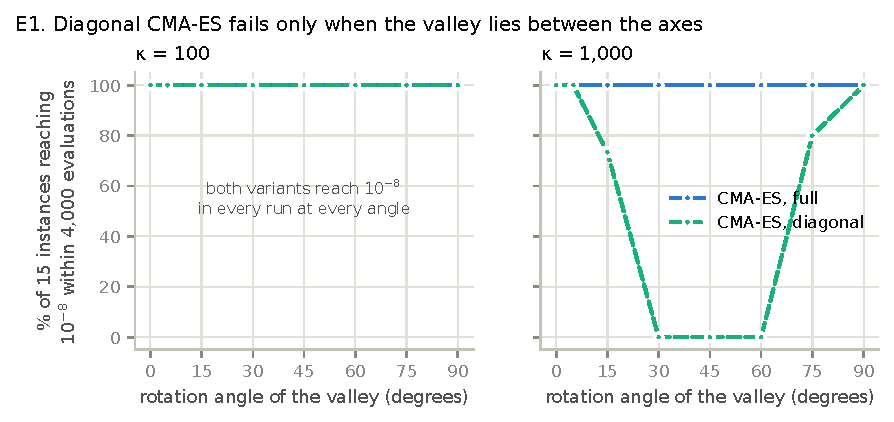
\includegraphics[width=0.78\linewidth]{figures/geom_e1_angle.pdf}
\caption{Part B, E1. Success of full (solid) and diagonal (dashed) CMA-ES against the angle of a 2-D valley.}
\label{fig:e1}
\end{figure}

\textbf{BO: a negative result, diagnosed.} Reading the fitted kernel directly, ARD's long axis is off by exactly
$45^\circ$ on $45^\circ$ problems while the full metric is within $0.2^\circ$--$4^\circ$. Yet the first head-to-head
showed \emph{no} rotation penalty for BO-ARD ($+0.05$ \ci{-0.53}{+0.63} decades at $\kappa=100$), while diagonal
CMA-ES paid $+1.70$ \ci{+0.41}{+2.57}. BO was stalling everywhere, near $10^{-2.6}$ even on the round bowl.
Per-iteration logs ruled out the target transform's floor and the candidate search, and showed the cause: the
GP fitted a noise term to a noise-free function and explained its best points away as noise (fitted noise SD
0.2--0.4; posterior mean at the incumbent 2--2.5$\times$ the gap to the second-best point above its observed value),
so EI against the observed best underflowed below $10^{-12}$ in 97--100\% of late iterations. Fixing the noise
variance at $10^{-6}$ lifted BO by $-1.17$ \ci{-1.71}{-0.74} decades; LogEI \citep{ament2023logei}, which fixes the
underflow but not its cause, changed nothing ($+0.01$ \ci{-0.79}{+0.47}).

\textbf{The penalty, once BO works.} Re-running the 180 BO runs with the fix, paired by instance, the negative
result reversed (Fig.~\ref{fig:pen}): BO-ARD's rotation penalty became $+2.01$ \ci{+1.28}{+2.97} decades at
$\kappa=10^4$ and BO-full's stayed non-significant. Table~\ref{tab:robust} repeats the key comparison with a second
kernel (Mat\'ern-5/2), a second acquisition search (200 extra candidates around the incumbent) and a TuRBO-style
trust region whose box is either axis-aligned with ARD-scaled sides, as published, or rotated to the full
metric: in every variant the axis-restricted version ends significantly behind on rotated problems and level on
aligned ones. With the trust region, BO also beats full CMA-ES at 200 evaluations on aligned $\kappa=100$ ($-1.36$
\ci{-2.02}{-0.85}) and rotated $\kappa=10^4$ ($-3.32$ \ci{-4.24}{-1.82}); with plain EI, CMA-ES wins by 200 evaluations
at $\kappa\le100$ (1.2--2.7 decades).

\begin{figure}[t]
\centering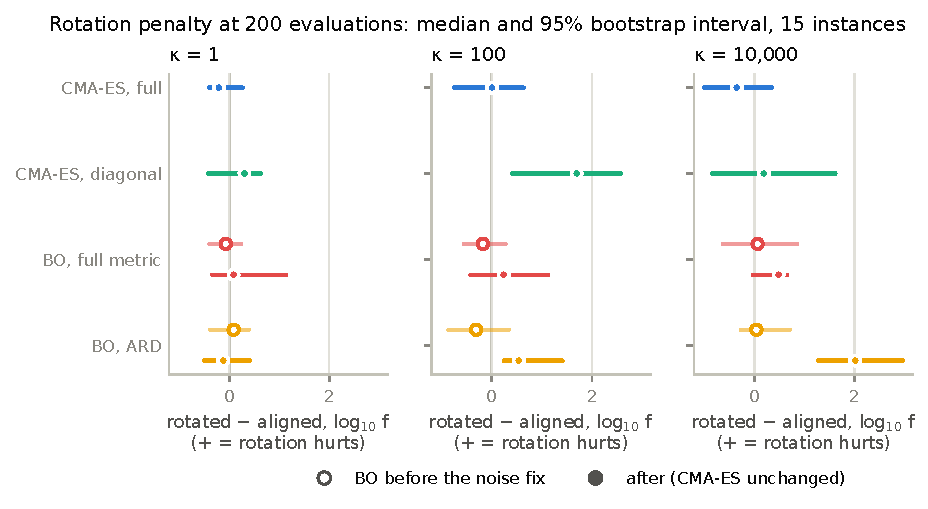
\includegraphics[width=0.86\linewidth]{figures/geom_rotation_penalty.pdf}
\caption{Part B. Rotation penalty at 200 evaluations (median, 95\% bootstrap interval, 15 instances). Hollow: BO
before the noise fix. The axis-restricted variant pays in both families once BO is no longer stalled.}
\label{fig:pen}
\end{figure}

\begin{table}[t]
\centering\small
\begin{tabular}{lcc}
\toprule
BO variant (2-D, 15 instances, 200 evaluations) & rotated $\kappa=10^4$ & aligned $\kappa=10^4$ \\
\midrule
EI, squared exponential, noise fixed & $+1.40$ \ci{+0.68}{+1.69} & $-0.13$ \ci{-1.15}{+0.19} \\
EI, Mat\'ern-5/2 & $+1.06$ \ci{+0.59}{+1.43} & $-0.13$ \ci{-0.70}{+0.54} \\
EI + local candidates & $+1.28$ \ci{+0.12}{+2.36} & $-2.96$ \ci{-3.44}{+2.61} \\
Trust region, ARD box vs rotated box & $+2.92$ \ci{+1.27}{+3.79} & $-0.39$ \ci{-3.11}{+4.65} \\
\bottomrule
\end{tabular}
\caption{Part B. Axis-restricted minus tilting version, median $\log_{10}f$ at 200 evaluations, paired by instance
(+ = axis-restricted worse). Wide aligned intervals come from the boundary trap (text).}
\label{tab:robust}
\end{table}

\textbf{Beyond the quadratic.} A quadratic has the same orientation everywhere; Rosenbrock (COCO f8/f9
\citep{hansen2009bbobfunctions}) bends, so its local orientation changes along the path, and even ``aligned'' f8
is tilted $63.5^\circ$ near its optimum. With 4,000 evaluations full CMA-ES reaches $10^{-5}$ in every run (median
about 500 evaluations), diagonal in 0\% (f8) and 27\% (f9): what matters is the local orientation. For BO (300
evaluations) the trust region beats plain BO by 3.5--3.7 decades and its tilted box beats the axis-aligned one by
2.0--2.5 decades, even on f8. We predicted that fitting the GP only to points inside the region would follow the
bend better; it was 1.8--2.0 decades \emph{worse}, and worse still (2.7) on a quadratic control where local and
global shape coincide, so the loss is discarded data, not geometry.

\textbf{Invariances, units, boundaries.} CMA-ES runs were bit-identical to the baseline under every monotone
transformation of $f$ (120/120); BO is not rank-invariant, and cubing $f$ costs it 1.7 decades through its relative
target floor. A change of units hurts every method with default set-ups (CMA-ES about 3.9 decades, BO 1.3--1.4);
mapping CMA-ES's initial covariance as Hansen requires ($C_0=S^{-2}$) restores invariance. BO over-samples the box
edge \citep{siivola2018boundary}: it is 1.62 / 0.73 decades worse when the optimum lies 0.1 inside an edge and better
when it lies on it. Combined with search around the incumbent this produces a \emph{boundary trap}: 4--8 of 15 runs per
aligned ill-conditioned cell stall on the valley floor at the box edge. In those runs about two random candidates per
iteration are truly better, yet the GP gives them EI near $10^{-34}$: a model failure. Reflecting out-of-box
candidates instead of clipping them removes the trap for the trust region (6 and 4 stuck runs to 0) but not for local
candidates.

\textbf{Noise.} On the $\kappa=100$ quadratic with additive noise $\sigma\in\{0.01,0.1,1\}$ and every recommendation
scored on the noise-free $f$, BO's posterior-mean pick beats its lowest reading by up to 1.08 decades, CMA-ES's mean
helps only with a larger population ($\lambda=24$), and spending evaluations on repeats or a final re-evaluation
reserve did not pay at 200 evaluations. With each family's best settings the two are level at every noise level.
The one anomaly, a worse model-based pick with replicates, is again the noise-fitting GP: a correctly specified GP
on the raw values never does worse than the lowest reading.

%=====================================================================
\section{Synthesis: what the two parts establish together}\label{sec:synth}
%=====================================================================
%% AUTHORS: joint section, rewrite together.
\textbf{Shape and scale both decide success, within each family.} Part A shows that a model with the wrong
\emph{scale} fails to find or to refine a narrow basin, and Part B that a model restricted in \emph{shape} fails on
tilted valleys in both families. In neither part does the family alone predict the outcome: diagonal and full
CMA-ES differ by up to 100 percentage points on the same rotated problem, and capped and default BO by 43 successes out of 50
on the same landscape (44 against 1 on fresh seeds).

\textbf{BO's decisive fixes were to the model fit, not the acquisition.} Independently, both parts found BO
failing because its GP was mis-fitted, and both found acquisition changes nearly powerless: in Part A the lengthscale
ran to its bound (capping it took success from 5 to 39/50; $\xi$, LCB and Thompson sampling at most 17/50), in Part B
the fitted noise absorbed the best points (fixing it gained over a decade; LogEI nothing). In both, BO's
results depend on implementation choices that published defaults leave open.

\textbf{CMA-ES adapts shape well but must commit to a scale.} One step size cannot both find a distant basin and refine a
narrow one (Part A), but its covariance follows a rotated valley reliably (Part B); population size and restarts,
which change only how much is sampled, did not move success on the primary landscape.

\textbf{Trade-offs.} BO leads early in both parts and costs roughly $10^5$ times more computation per run; settings
that help on the hard landscape cost on easy ones (the cap on the sphere, tilting on aligned problems); and BO's
boundary preference appears in both parts (edge sampling under large $\xi$; the boundary trap).

\textbf{Limitations.} All headline results are 2-D, so dimension effects are inferred (for CMA-ES) rather than
measured for BO. Each part rests on few landscapes (ellipsoids and Rosenbrock; one primary landscape plus two validation
functions) and 15--50 seeds, which leaves some differences unresolved. BO results reproduce in distribution only: long
BO runs are not bit-repeatable even with one BLAS thread. Some follow-ups were added after seeing results and are
labelled as such; untested mechanisms are stated as hypotheses.

\small
\bibliographystyle{abbrvnat}
\bibliography{references}

\end{document}
